% --------------------------------------------------------------
% This is all preamble stuff that you don't have to worry about.
% Head down to where it says "Start here"
% --------------------------------------------------------------

\documentclass[12pt]{article}


\usepackage[utf8]{inputenc}
\usepackage{intmacros}
\usepackage[margin=1in]{geometry} 
\usepackage{amsmath,amsthm,amssymb}
\usepackage[backend=biber, style=ieee, isbn=false,sortcites, maxbibnames=5, minbibnames=1]{biblatex}
\usepackage{hyperref}
\usepackage{xcolor}
\usepackage{amsmath}
\usepackage{graphicx}
\usepackage{caption,subcaption}
\captionsetup{labelsep = period} % Figure 2. Caption (rather than Figure 2: Caption)

\usepackage[]{hyperref}
\hypersetup{
	colorlinks   = true, %Colours links instead of ugly boxes
	urlcolor     = blue, %Colour for external hyperlinks
	linkcolor    = red, %Colour of internal links
	citecolor   = green %Colour of citations
}
\addbibresource{bibliography.bib}


%\newenvironment{theorem}[2][Theorem]{\begin{trivlist}
%		\item[\hskip \labelsep {\bfseries #1}\hskip \labelsep {\bfseries #2.}]}{\end{trivlist}}
%\newenvironment{lemma}[2][Lemma]{\begin{trivlist}
%		\item[\hskip \labelsep {\bfseries #1}\hskip \labelsep {\bfseries #2.}]}{\end{trivlist}}
%\newenvironment{exercise}[2][Exercise]{\begin{trivlist}
%		\item[\hskip \labelsep {\bfseries #1}\hskip \labelsep {\bfseries #2.}]}{\end{trivlist}}
%\newenvironment{reflection}[2][Reflection]{\begin{trivlist}
%		\item[\hskip \labelsep {\bfseries #1}\hskip \labelsep {\bfseries #2.}]}{\end{trivlist}}
%\newenvironment{proposition}[2][Proposition]{\begin{trivlist}
%		\item[\hskip \labelsep {\bfseries #1}\hskip \labelsep {\bfseries #2.}]}{\end{trivlist}}
%\newenvironment{corollary}[2][Corollary]{\begin{trivlist}
%		\item[\hskip \labelsep {\bfseries #1}\hskip \labelsep {\bfseries #2.}]}{\end{trivlist}}
% OPERATORS

\newcommand{\norm}[1]{\left\lVert#1\right\rVert_2}

\newcommand{\indicator}{\mathbb{I}} 
\newcommand{\bs}{\boldsymbol}

%\DeclareMathOperator*{\argmax}{arg\,max}
%\DeclareMathOperator*{\argmin}{arg\,min}

\begin{document}
	
% --------------------------------------------------------------
%                         Start here
% --------------------------------------------------------------

%\renewcommand{\qedsymbol}{\filledbox}

\title{Assignment 2: HMM for Categorical Data Sequences}%
\author{Daniel Barrejón Moreno} %if necessary, replace with your course title

\maketitle

In this project we will develop a EM Baum-Welch algorithm for training HMM for the available data set, which are sequences of documents. The goal is to find the states or topics each document belongs to. In the following we will derive the equations and finally we will present the different results we obtained for different number of topics.
\section{Complete data log-likehood $l_{c}\left(\boldsymbol\theta\right)$ for the N sequences}
The complete data log-likelihood has the following form
\begin{equation}
\label{ll1}
l_{c}\left(\boldsymbol\theta\right) = \log p ( S , Y | \boldsymbol\theta ) = \log \prod _ { n = 1 } ^ { N } \left( p \left( s _ { 1 } ^ { n } | \boldsymbol\pi \right) \prod _ { t = 2 } ^ { T _ { n } } p \left( s _ { t } ^ { n } | s _ { t - 1 } ^ { n } , \mathbf { A } \right) \right) \left( \prod _ { t = 1 } ^ { T _ { n } } p \left( \mathbf { y } _ { t } ^ { n } | s _ { t } ^ { n } , \mathbf { B } \right) \right),
\end{equation}
where $\log$ operator is the Naperian logarithm, $S$ represents the hidden states of the model, $Y$ is the observed continuous sequence, $\mathbf { A }$ stands for the state transition probabilities,$B$ the observatoin emission probabilities and $\boldsymbol\pi$ is the initial state probability distribution.\\
\noindent The parameters of the model are
\begin{equation}
\boldsymbol\theta = \{ \mathbf { A } , \mathbf { B } , \boldsymbol\pi \},
\end{equation}
where $\mathbf { A }$  is the state transition matrix, $\mathbf { B } $ is the emission matrix and  $\boldsymbol\pi $ represents the probability of each state. In Equation \ref{ll1} we can distinguish three main terms: the $\boldsymbol\pi$, $\mathbf { A }$ and $\mathbf { B } $ ones which can be rewritten as
\begin{align}
p \left( s _ { 1 } ^ { n } | \boldsymbol\pi \right) &= \prod\limits_{k=1}^{K}\pi_{k}^{\indicator \lbrace s_{1}^{n}=k|Y,\boldsymbol\theta\rbrace},\\
p \left( s _ { t } ^ { n } | s _ { t - 1 } ^ { n } , \mathbf { A } \right) &= \prod\limits_{k=1}^{K} \prod\limits_{k'=1}^{K}a_{k,k'}^{\indicator \lbrace s_{t-1}^{n}=k,s_{t}^{n}=k'|Y,\boldsymbol\theta\rbrace},\\
p \left( \mathbf { y } _ { t } ^ { n } | s _ { t } ^ { n } , \mathbf { B } \right) &= \prod\limits_{k=1}^{K} p \left( \mathbf { y } _ { t } ^ { n } | \boldsymbol b_{k} \right) = \prod\limits_{k=1}^{K} p \left( \mathbf { y } _ { t } ^ { n } | \boldsymbol\theta_{k} \right) \label{p3LL}.
\end{align}
In this case, $\indicator$ represents an indicator function, $k = \lbrace{1,...,K}\rbrace$ the current latent state of the model, $a_{k,k'}$ the $k$th row and $k'$th column element of the forementioned matrix $\mathbf { A }$ and $t = \lbrace{1,...,T_{n}}\rbrace$ the position of the state in sequence $n$. In order to have a similar notation as the one used in Assignment 1,  $\mathbf{b}_{k}$ (that belonged to $\mathbf{B}$) becomes $\boldsymbol\theta_{k}$, which represents the categories of the topic $k$ for the categorical distribution.\\

\noindent Since our data follow a categorical distribution, Equation \ref{p3LL} can be expressed as
\begin{equation}
p \left( \mathbf { y } _ { t } ^ { n } | \boldsymbol\theta_{k} \right) = \prod\limits_{j=1}^{Dt} \text{Cat}(y_{j,t}|\boldsymbol\theta_{k}),
\end{equation}
and with further development we can get the following expression
\begin{equation}
p \left( \mathbf { y } _ { t } ^ { n } | \boldsymbol\theta_{k} \right) = \prod\limits_{j=1}^{Dt} \text{Cat}(y_{j,t}|\boldsymbol\theta_{k}) = \prod\limits_{m=1}^{I}\prod\limits_{j=1}^{Dt}\theta_{k,m}^{\indicator\lbrace{y_{j,t}^{n}=m}\rbrace} = \prod\limits_{m=1}^{I}\theta_{k,m}^{\sum\limits_{j=1}^{Dt}\indicator\lbrace{y_{j,t}^{n}=m}\rbrace} = \prod\limits_{m=1}^{I}\theta_{k,m}^{\mu^{n}_{t,m}},
\end{equation}
where  $\mu^{n}_{t,m}$ is denoted as follows
\begin{equation}
\mu^{n}_{t,m} = \sum\limits_{j=1}^{Dt}\indicator\lbrace{y_{j,t}^{n}=m}\rbrace.
\end{equation}
Finally, the expression of the complete data log-likelihood can be expressed in the following form	
\begin{equation}
\begin{split}
l_{c}\left(\boldsymbol\theta\right) &= \sum\limits_{n=1}^{N}\sum\limits_{k=1}^{K}\indicator \lbrace s_{1}^{n}=k|Y,\boldsymbol\theta\rbrace \log(\pi_{k}) + \\
&+ \sum\limits_{n=1}^{N}\sum\limits_{k=1}^{K}\sum\limits_{k'=1}^{K}\sum\limits_{t=1}^{T_{n}}\indicator \lbrace s_{t-1}^{n}=k,s_{t}^{n}=k'|Y,\boldsymbol\theta\rbrace \log(a_{k,k'}) + \\
&+ \sum\limits_{n=1}^{N}\sum\limits_{t=1}^{T_{n}}\indicator \lbrace s_{t}^{n}=k|Y,\boldsymbol\theta\rbrace \sum\limits_{m=1}^{I}\mu^{n}_{t,m} \log(\theta_{k,m}).
\end{split}
\end{equation}

\section{Expected Complete Data Logl-likelihood $Q \left( \boldsymbol { \theta } , \boldsymbol { \theta } ^ { t - 1 } \right)$}
The expected complete data log-likelihood has the following form
\begin{equation}
Q \left( \boldsymbol { \theta } , \boldsymbol { \theta } ^ { t - 1 } \right) = E \left\{ l _ { c } ( \boldsymbol { \theta } ) | \mathcal { D } , \boldsymbol { \theta } ^ { t - 1 } \right\}
\end{equation}
As in the previous section, and considering the nature of $l_{c}$ and its three main components, this expectation calculation can be divided in three.
\begin{align}
& \expectation \left( \sum _ { n = 1 } ^ { N } \indicator \left( s _ { 1 } ^ { n } = k | Y , \bs\theta \right) \right) = \sum _ { n = 1 } ^ { N } \gamma _ { n , 1 } ( k ), \\
& \expectation \left( \sum _ { n = 1 } ^ { N } \sum _ { t = 2 } ^ { T _ { n } } \indicator \left( s _ { t - 1 } ^ { n } = k , s _ { t } ^ { n } = k' | Y , \bs\theta \right) \right) = \sum _ { n = 1 } ^ { N } \sum _ { t = 2 } ^ { T _ { n } } \xi _ { n , t } ( k , k' ), \\
& \expectation \left( \sum _ { n = 1 } ^ { N } \sum _ { t = 1 } ^ { T _ { n } } \indicator \left( s _ { t } ^ { n } = k | Y , \bs\theta \right) \right) = \sum _ { n = 1 } ^ { N } \sum _ { t = 1 } ^ { T _ { n } } \gamma _ { n , t } ( k ),
\end{align}
where it must be satisfied
\begin{equation}
\sum _ { k = 1 } ^ { K } \gamma _ { n , t } ( k ) = 1.
\end{equation}
\noindent The analogous backwards term for$ \gamma _ { n , t } ( k ) $ is denoted as $\xi _ { n,t } ( k , k' )$ 
\begin{equation}
\xi _ { n,t } ( k , k' ) = \alpha _ { t-1 }^{n} ( k ) a _ { k,k' } \prod\limits_{m=1}^{I} \theta_{k,m}^{\mu^{n}_{t,m}} \beta _ { t }^{n} ( k' ),
\end{equation}
and $ \gamma _ { n , t } ( k ) $
\begin{equation}\label{eq:gamma}
\gamma _ { n , t } ( k )\propto \beta _ { t }^{n} ( k )\alpha _ { t }^{n} ( k )
\end{equation}
The terms $\alpha$ and $\beta$ are computed by means of the \textbf{forward-backward algorithm }as follows
\begin{align}
\label{alfabeta}
&\alpha _ { 1 }^{n} ( k ) = \pi _ { k } \prod\limits_{m=1}^{I}\theta_{k,m}^{\mu^{n}_{1,m}}, \\
&\alpha _ { t }^{n} ( k ) = \left( \sum _ { k' = 1 } ^ { K } \alpha _ { t - 1 }^{n} ( k' ) a _ { k',k } \right) \prod\limits_{m=1}^{I}\theta_{k,m}^{\mu^{n}_{t,m}}, \\
&\beta _ { T_{n} }^{n} ( k ) = 1, \\
& \beta _ { t }^{n} ( k ) = \sum _ {k' = 1 } ^ { K } a _ { k,k'}  \prod\limits_{m=1}^{I}\theta_{k',m}^{\mu^{n}_{t+1,m}}  \beta _ { t + 1 }^{n} ( k' ).
\end{align}
The development above yields the final expression for $Q \left( \boldsymbol { \theta } , \boldsymbol { \theta } ^ { t - 1 } \right)$
\begin{equation}
\begin{split}
Q \left( \boldsymbol { \theta } , \boldsymbol { \theta } ^ { t - 1 } \right) &= \sum\limits_{k=1}^{K}\sum _ { n = 1 } ^ { N } \gamma _ { n , 1 } ( k ) \log(\pi_{k}) + \\
&+ \sum\limits_{k=1}^{K}\sum\limits_{k'=1}^{K}\sum _ { n = 1 } ^ { N } \sum _ { t = 2 } ^ { T _ { n } } \xi _ { n , t } ( k , k' ) \log(a_{k,k'}) + \\
&+ \sum\limits_{k=1}^{K}\sum\limits_{m=1}^{I}\sum _ { n = 1 } ^ { N } \sum _ { t = 1 } ^ { T _ { n } } \gamma _ { n , t } ( k )\mu^{n}_{t,m} \log(\theta_{k,m}).
\end{split}
\end{equation}
\section{ML Inference}
In this section we develop the update formulas for the model, which are $\mathbf{A}$, $\bs\theta$ and $\bs\pi$. These will be computed using Lagrange-Multipliers.
\subsection{ML estimation of $\pi_{k}$}
In order to compute $\pi_{k}$, we first need to take into account the following restrictions
\begin{align}
& 0 \leq \pi_{k} \leq 1 \\
& \sum\limits_{k = 1}^{K} \pi_{k} = 1.
\end{align}
Now, let us define the Lagrangian as
\begin{equation}
\label{lagrange_pik}
L\left( Q(\pi_{k}),\lambda \right) = Q(\pi_{k}) + \lambda \left( \sum \limits_{k=1}^{K} \pi_{k} - 1 \right),
\end{equation}
which will be optimized in this way
\begin{equation}
\label{minmax_lagrange_pik}
\min_{\substack{\lambda}} \max_{\substack{\pi_{k}}} \lbrace L\left( Q(\pi_{k}),\lambda \right) \rbrace.
\end{equation}
We first take the derivative with respect to $\pi_{k}$ and equating it to 0
\begin{equation}
\label{deriv_pik}
\begin{split}
& \dfrac{\partial L}{\partial \pi_{k}} = \sum \limits_{n=1}^{N} \dfrac{\gamma_{n,1}(k)}{\pi_{k}} - \lambda = 0, \\
& \pi_{k} = \dfrac{1}{\lambda} \sum \limits_{n=1}^{N} \gamma_{n,1}(k).
\end{split}
\end{equation}
Now, with respect to $\lambda$
\begin{equation}
\begin{split}
& \dfrac{\partial L}{\partial \lambda} = \sum \limits_{k=1}^{K} \pi_{k} - 1 = 0,\\
& \sum \limits_{k=1}^{K} \pi_{k} = 1.\\
\end{split}
\end{equation}
Taking into account the previous equation, if in both sides of Equation \ref{deriv_pik} summatories all over $K$ are taken, then the value of $\lambda$ can be obtained
\begin{equation}
\begin{split}
& \sum \limits_{k=1}^{K}\pi_{k} = \sum \limits_{k=1}^{K} \dfrac{1}{\lambda} \sum \limits_{n=1}^{N} \gamma_{n,1}(k)\\
& 1 = \dfrac{1}{\lambda} \sum \limits_{n=1}^{N}\sum \limits_{k=1}^{K}\gamma_{n,1}(k).\\
\end{split}
\end{equation}
Now, considering the previously imposed restrictions and recalling that
\begin{equation}
\sum _ { k = 1 } ^ { K } \gamma _ { n , t } ( k ) = 1,
\end{equation}
the value of $\lambda$ is
\begin{equation}
\begin{split}
& 1 = \dfrac{1}{\lambda} \sum \limits_{n=1}^{N}1.\\
& \lambda = N.\\
\end{split}
\end{equation}
And with that value of $\lambda$ the estimated value of $\pi_{k}$ is
\begin{equation}
\widehat{\pi}_{k} = \dfrac{1}{N} \sum \limits_{n=1}^{N} \gamma_{n,1}(k).
\end{equation}
\subsection{ML estimation of $\theta_{k,m}$}
Now, the parameter to be estimated is $\theta_{k,m}$ and the constraint is now
\begin{equation}
\label{constraint_thetakm}
\sum \limits_{m=1}^{I} \theta_{k,m} = 1.
\end{equation}
In this case, the expression for the Lagrangian has the following form
\begin{equation}
\label{lagrange_thetakm}
L\left( Q(\theta_{k,m}),\lambda \right) = Q(\theta_{k,m}) + \lambda \left( \sum \limits_{m=1}^{I} \theta_{k,m} - 1 \right),
\end{equation}
which will be optimized in this way
\begin{equation}
\label{minmax_lagrange_thetakm}
\min_{\substack{\lambda}} \max_{\substack{\theta_{k,m}}} \lbrace L\left( Q(\theta_{k,m}),\lambda \right) \rbrace.
\end{equation}
By first taking the derivative with respect to $\theta_{k,m}$ and equating it to 0
\begin{equation}
\label{deriv_thetakm}
\begin{split}
& \dfrac{\partial L}{\partial \theta_{k,m}} = \sum \limits_{n=1}^{N}\sum _ { t = 1 } ^ { T _ { n } } \dfrac{\gamma_{n,t}(k)\mu_{t,m}^{n}}{\theta_{k,m}} - \lambda  = 0 , \\
& \theta_{k,m} = \dfrac{1}{\lambda} \sum \limits_{n=1}^{N} \sum _ { t = 1 } ^ { T _ { n } }\gamma_{n,t}(k)\mu_{t,m}^{n}.
\end{split}
\end{equation}
And later with respect to $\lambda$
\begin{equation}
\begin{split}
& \dfrac{\partial L}{\partial \lambda} = \sum \limits_{m=1}^{I} \theta_{k,m} - 1 = 0,\\
& \sum \limits_{m=1}^{I} \theta_{k,m} = 1.\\
\end{split}
\end{equation}
Taking into account the previous equation, if in both sides of Equations \ref{deriv_thetakm} summatories all over $I$ are taken, then the value of $\lambda$ can be obtained
\begin{equation}
\begin{split}
& \sum \limits_{m=1}^{I}\theta_{k,m} = \sum \limits_{m=1}^{I} \dfrac{1}{\lambda} \sum \limits_{n=1}^{N}\sum _ { t = 1 } ^ { T _ { n } } \gamma_{n,t}(k)\mu_{t,m}^{n}\\
& 1 = \dfrac{1}{\lambda} \sum \limits_{n=1}^{N}\sum _ { t = 1 } ^ { T _ { n } }\sum \limits_{m=1}^{I}\gamma_{n,t}(k)\mu_{t,m}^{n},\\
& \lambda = \sum \limits_{n=1}^{N}\sum \limits_{ t = 1 } ^ { T _ { n }}\sum \limits_{m=1}^{I}\gamma_{n,t}(k)\mu_{t,m}^{n}.\\
\end{split}
\end{equation}
And with that value of $\lambda$ the estimated value of $\theta_{k,m}$ is
\begin{equation}
\widehat{\theta}_{k,m} = \dfrac{\sum \limits_{n=1}^{N} \sum \limits_ { t = 1 } ^ { T _ { n } }\gamma_{n,t}(k)\mu_{t,m}^{n}}{\sum \limits_{n=1}^{N}\sum \limits_ { t = 1 } ^ { T _ { n } }\sum \limits_{m=1}^{I}\gamma_{n,t}(k)\mu_{t,m}^{n}}.
\end{equation}
\subsection{ML estimation of $a_{k,k'}$}
The last parameter to be estimated is $a_{k,k'}$. The constraint is now
\begin{equation}
\label{constraint_akk}
\sum \limits_{k'=1}^{K} a_{k,k'} = 1.
\end{equation}
The Lagrangian will follow this expression
\begin{equation}
\label{lagrange_akk}
L\left( Q(a_{k,k'}),\lambda \right) = Q(a_{k,k'}) + \lambda \left( \sum \limits_{k'=1}^{K} a_{k,k'} - 1 \right),
\end{equation}
which will be optimized in this way
\begin{equation}
\label{minmax_lagrange_akk}
\min_{\substack{\lambda}} \max_{\substack{a_{k,k'}}} \lbrace L\left( Q(a_{k,k'}),\lambda \right) \rbrace.
\end{equation}
By first taking the derivative with respect to $a_{k,k'}$ and equating it to 0
\begin{equation}
\label{deriv_akk}
\begin{split}
& \dfrac{\partial L}{\partial a_{k,k'}} = \sum \limits_{n=1}^{N}\sum _ { t = 2 } ^ { T _ { n } } \dfrac{\xi_{n,t}(kk')}{a_{k,k'}} - \lambda = 0, \\
& a_{k,k'} = \dfrac{1}{\lambda} \sum \limits_{n=1}^{N} \sum _ { t = 2 } ^ { T _ { n } }\xi_{n,t}(kk').
\end{split}
\end{equation}
And later with respect to $\lambda$
\begin{equation}
\begin{split}
& \dfrac{\partial L}{\partial \lambda} = \sum \limits_{m=1}^{I} a_{k,k'} - 1 = 0 ,\\
& \sum \limits_{k'=1}^{K} a_{k,k'} = 1.\\
\end{split}
\end{equation}
Taking into account the previous equation, if in both sides of \eqref{deriv_akk} summatories all over $I$ are taken, then the value of $\lambda$ can be obtained
\begin{equation}
\begin{split}
& \sum \limits_{k'=1}^{K}a_{k,k'} = \sum \limits_{k'=1}^{K} \dfrac{1}{\lambda} \sum \limits_{n=1}^{N}\sum _ { t = 1 } ^ { T _ { n } } \xi_{n,t}(k,k')\\
& 1 = \dfrac{1}{\lambda} \sum \limits_{n=1}^{N}\sum _ { t = 1 } ^ { T _ { n } }\sum \limits_{k'=1}^{K}\xi_{n,t}(k,k'),\\
& \lambda = \sum \limits_{n=1}^{N}\sum \limits_{ t = 1 } ^ { T _ { n }}\sum \limits_{k'=1}^{K}\xi_{n,t}(k,k').\\
\end{split}
\end{equation}
And with that value of $\lambda$ the estimated value of $a_{k,k'}$ is
\begin{equation}
\widehat{a}_{k,k'} = \dfrac{\sum \limits_{n=1}^{N} \sum \limits_ { t = 1 } ^ { T _ { n } }\xi_{n,t}(k,k')}{\sum \limits_{n=1}^{N}\sum \limits_ { t = 1 } ^ { T _ { n } }\sum \limits_{k'=1}^{K}\xi_{n,t}(k,k')}.
\end{equation}

\section{State Decoder}
Each document in each sequence has been generated by some state of the HMM. In the following section we present the two types of decoding algorithms that have been used to find such states: the state-by-state MAP decoding based on the Forward-Backwards algorithm and the ML iterative Viterbi algorithm.

\subsection{MAP decoding based on Forward-Backwards}
In order to determine the state of each document for the different sequences we obtain the most probable state for each document at each sequence from the parameter $\gamma _ { n , t } ( k )$ which is computed in the E-step of the Baum-Welch EM using Equation \ref{eq:gamma}.

\subsection{ML Viterbi decoding}
As a comparison for the MAP decoding comment above, we have also implemented a Viterbi decoder. The Viterbi decoder is a dynamic programming algorithm for finding the most likely sequence of hidden states result of a sequence of observed events. Since we are dealing with hidden and observed states with HMM, the algorithm suits perfectly to our problem. The Viterbi decoding algorithm looks as follows
\begin{equation}
\underset { S } { \operatorname { argmax } } p ( S , Y ) = \underset { i } { \operatorname { argmax } } \left\{ \underset { s _ { 1 : T - 1 } } { \operatorname { argmax } } p \left( s _ { T } = i , s _ { 1 : T - 1 } , Y \right) \right\}.
\end{equation}
In particular, we will use an iterative implementation of the Viterbi Algorithm. For such implementation we define two iterative steps described below.

\begin{itemize}
	\item \textbf{Forward step}: Computed with the following equations
	\begin{align}
	\delta_{1}(k)&=\pi_{k} \prod\limits_{m=1}^{I}\theta_{k,m}^{\mu^{n}_{1,m}} \quad 1 \leq k \leq K\\
	\delta_{t}(k)&=\prod\limits_{m=1}^{I}\theta_{k,m}^{\mu^{n}_{t,m}} \max _{k'} a_{k',k} \delta_{t-1}(k') \quad 1 \leq k \leq K , 1 \leq t \leq T \\
	\varphi_{t}(k)&=\underset{k'}{\operatorname{argmax}} \hspace{0.1cm}a_{k',k} \delta_{t-1}(k') \quad 1 \leq k \leq K , 1 \leq t \leq T \\
	\end{align}
	\item \textbf{Backwards step}: The state estimation is computed using the following Equations
	\begin{align}
	\hat{\mathbf{s}}_{T}&=\underset{\boldsymbol{k}}{\arg \max } \delta_{T}(k)\\
	\hat{s}_{t}&=\varphi_{t+1}\left(\hat{s}_{t+1}\right)  1 \leq t \leq T.
	\end{align} 
\end{itemize}

\section{Experiments}
For the experiments conducted in this project the maximum number of iterations of the EM algorithm has been set to 100 iterations, the tolerance value has been set to $10^{-3}$ a total of 30 different initializations have been done. We have tested the system for different values of $K$, \emph{i.e.} $K = \{2,3,4,5\}$. For each of these experiments we will show the the best log-likelihood for the optimal initialization of the algorithm as well as $A$ and $\pi$. The matrix $\boldsymbol{\theta}$ that is actually the model parameter $\mathbf{B}$ has not been shown because the number of rows is equal to the length of the dictionary $I$ and displaying such matrix both in matrix form or with a colormap plot does not give much information of the emission probabilities. \\

\noindent One \textbf{important} aspect about the implementation of the algorithm is that instead of working with the actual $\xi _ { n,t } ( k , k' )$ we work with a similar implementation used in \cite{murphy2012machine}, which consider working with the expected sufficient statistics for the transition matrix, for a given observation sequence. This may be rewritten as follows
\begin{equation}
\xi_\Sigma(k,k^{\prime}) = \sum\limits_{t=2}^{T} p(S(t) = k, S(t+1) = k^{\prime} | y(1:T)),
\end{equation}
where the subscript $\Sigma$ indicates the sum over $t$. Notice that, for a given sequence, this matrix is no longer a tensor but a matrix of dimension $K\times K$.

\subsection{Simulations}
In Table \ref{tab:experiments} we can check the different reported values of $\mathbf{A}$ and $\pi$ for the different values of $k$.

\begin{table}[h]
	\hskip-2cm
	\begin{tabular}{|c|c|c|c|c|}
		\hline
		$K = $& 2 & 3 & 4 & 5 \\ \hline \hline
		$\mathbf{A}$     & $\begin{bmatrix}0.32 & 0.68\\0.37 & 0.63 \end{bmatrix} $ &  $\begin{bmatrix}0.64 & 0.18 & 0.18\\0.44 & 0.20 & 0.36\\0.38 & 0.44 & 0.18 \end{bmatrix}$  &$ \begin{bmatrix}0.2 & 0.27 & 0.43 & 0.1\\0.21 & 0.30 & 0.13 & 0.36\\0.1 & 0.35 & 0.34 & 0.21\end{bmatrix}  $  & $\begin{bmatrix}0.02 & 0.22 & 0.36 & 0.34 & 0.06\\0.07 & 0.16 & 0.21 & 0.21 & 0.35\\0.12 & 0.11 & 0.44 & 0.15 & 0.18\\0.32 & 0.22 & 0.35 & 0.1 & 0.01\\0.26 & 0.14 & 0.30 & 0.20 & 0.10 \end{bmatrix}   $ \\ \hline
		$\pi$ & $\begin{bmatrix}0.28 & 0.72\end{bmatrix} $  & $\begin{bmatrix}0.14 & 0.30 & 0.56\end{bmatrix} $  & $\begin{bmatrix}0.34 & 0.38 & 0.28 & 1.27e^{-80}\end{bmatrix} $   & $\begin{bmatrix}0.48 & 0.38 & 6.46e^{-80} & 1.12e^{-103} & 0.13\end{bmatrix} $  \\ \hline
	\end{tabular}
	\caption{Table for the different Experiments.}
	\label{tab:experiments}
\end{table}

The comparison of the log-likelihood for each value of $K$ is shown in Figure \ref{fig:ll_comparison}. As it can be seen, for greater values of $K$ the log-likelihood improves. From this behaviour we could infer that the optimal value is $K=5$. However, when we check the $\pi$ values for $K=4$ and $K=5$ at Table \ref{tab:experiments} we can see that there is one and two topics respectively whose influence on the documents is actually a really small value which can be approximated to 0. Therefore, we can conclude that, although for $K=5$ we get the optimal likelihood, actually when we observe the output result we could also conclude that $K=3$ might be also a good candidate.

\begin{figure}[h]
	\centering
	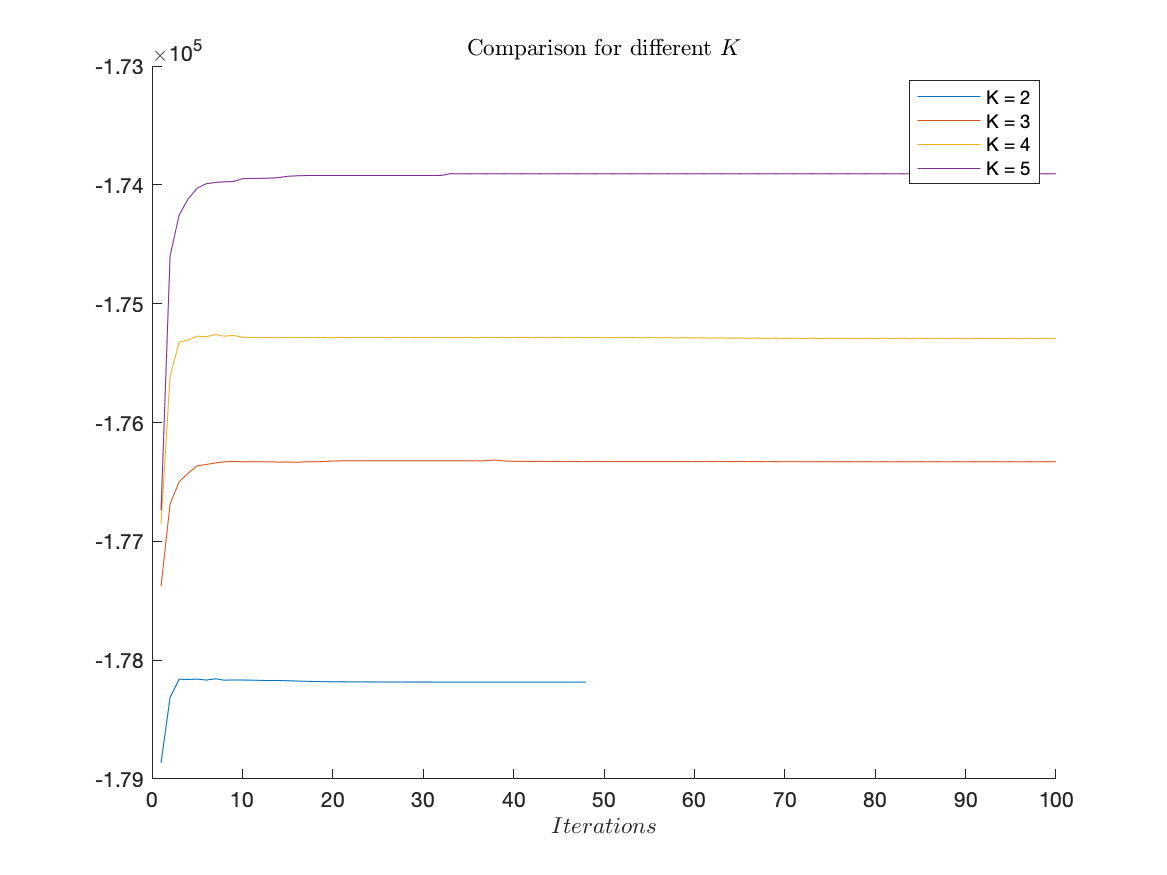
\includegraphics[width=0.8\textwidth]{images/ll_comparison.png}
	\caption{Comparison of the log-likelihoods for K $\in$ [2,5]}
	\label{fig:ll_comparison}
\end{figure}

In Figure \ref{fig:Q_all} we show individually each likelihood. As you might notice the likelihood always increases; however, when the curve gets to the 'plateau' behaviour, the likelihood tends to oscillate. This is due to the correction steps we are taking into account in the implementation of the code when trying to keep the parameters of the model which are probabilities within the range $\in (0,1)$. With some more depuration of the code this behaviour would disappear.\\

\begin{figure}[h]
	\centering
	\begin{subfigure}{0.45\textwidth}
		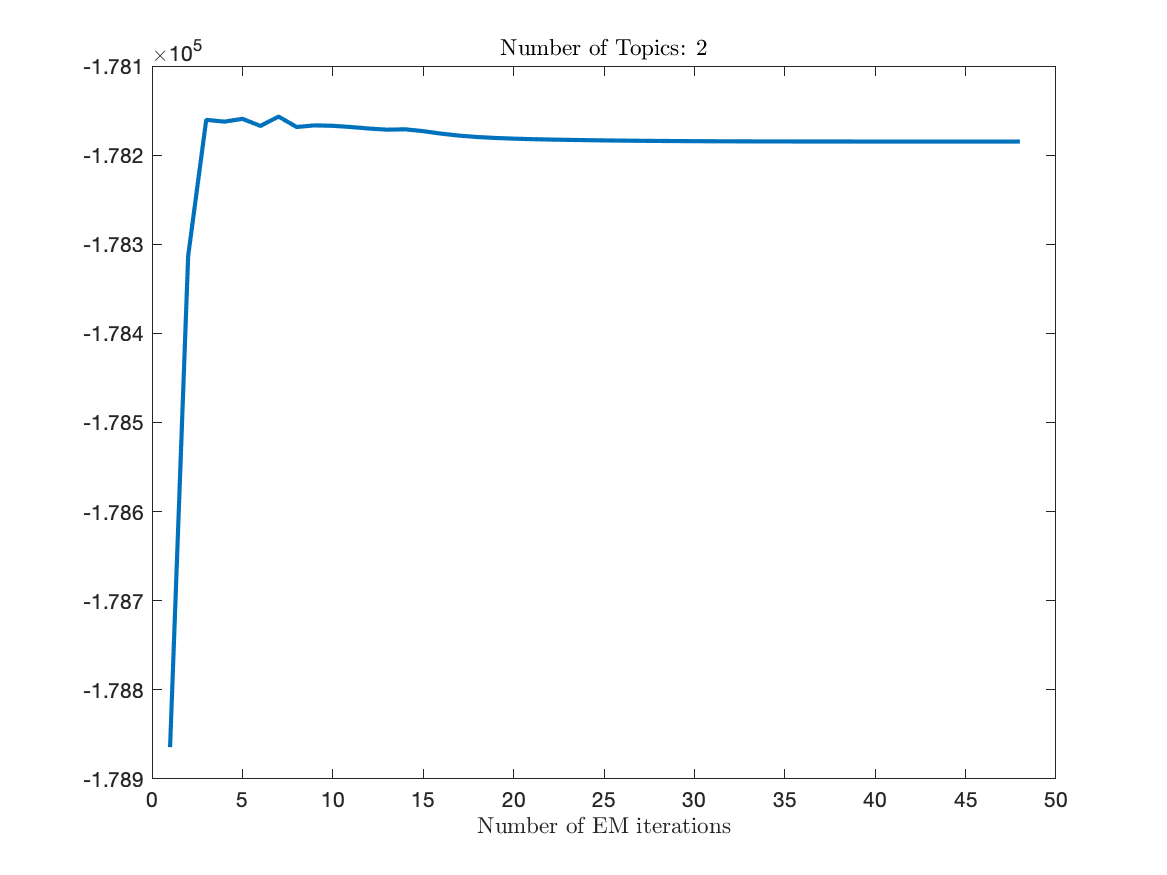
\includegraphics[width=\textwidth]{images/Q_2_topics.png}
		\caption{Log-likelihood curve for K = 2}
		\label{fig:Q2}
	\end{subfigure}
	~	
	\begin{subfigure}{0.45\textwidth}
		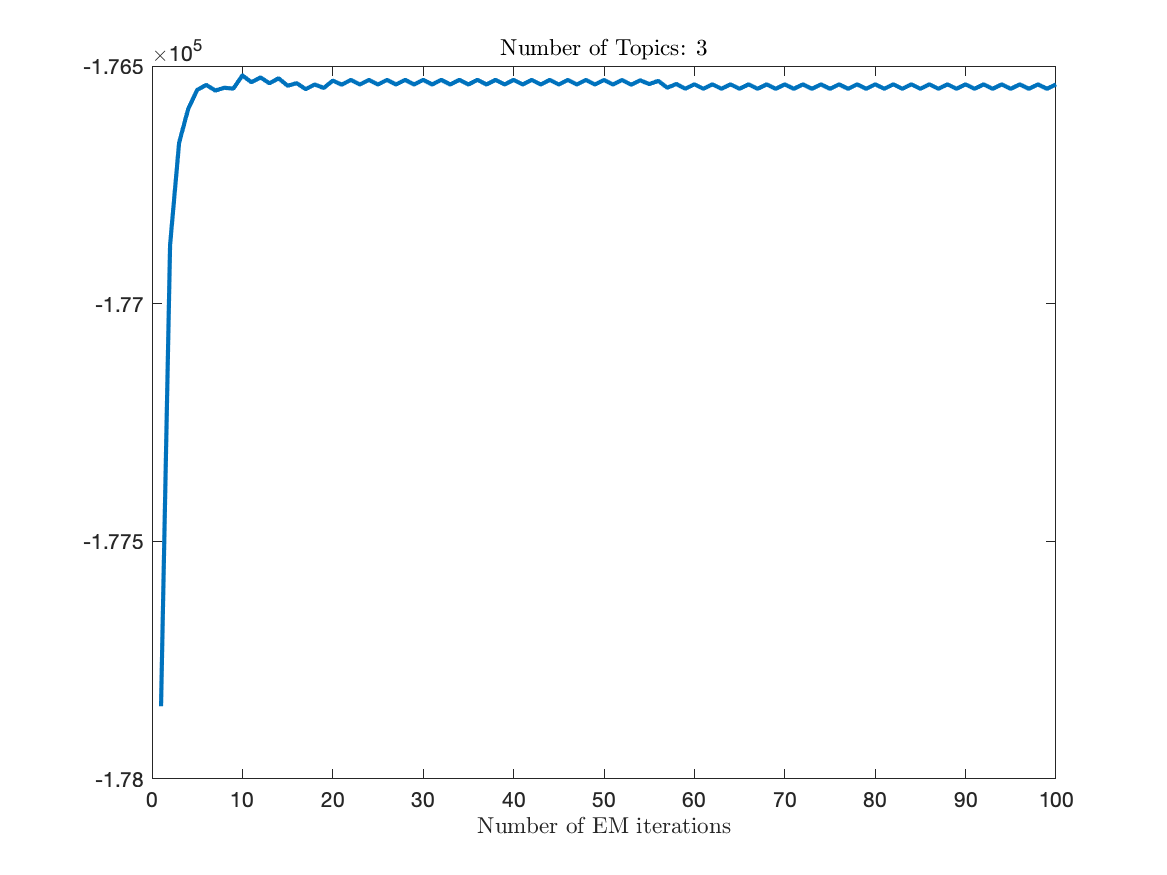
\includegraphics[width=\textwidth]{images/Q_3_topics.png}
		\caption{Log-likelihood curve for K = 3}
		\label{fig:Q3}
	\end{subfigure}
	~	
	\begin{subfigure}{0.45\textwidth}
		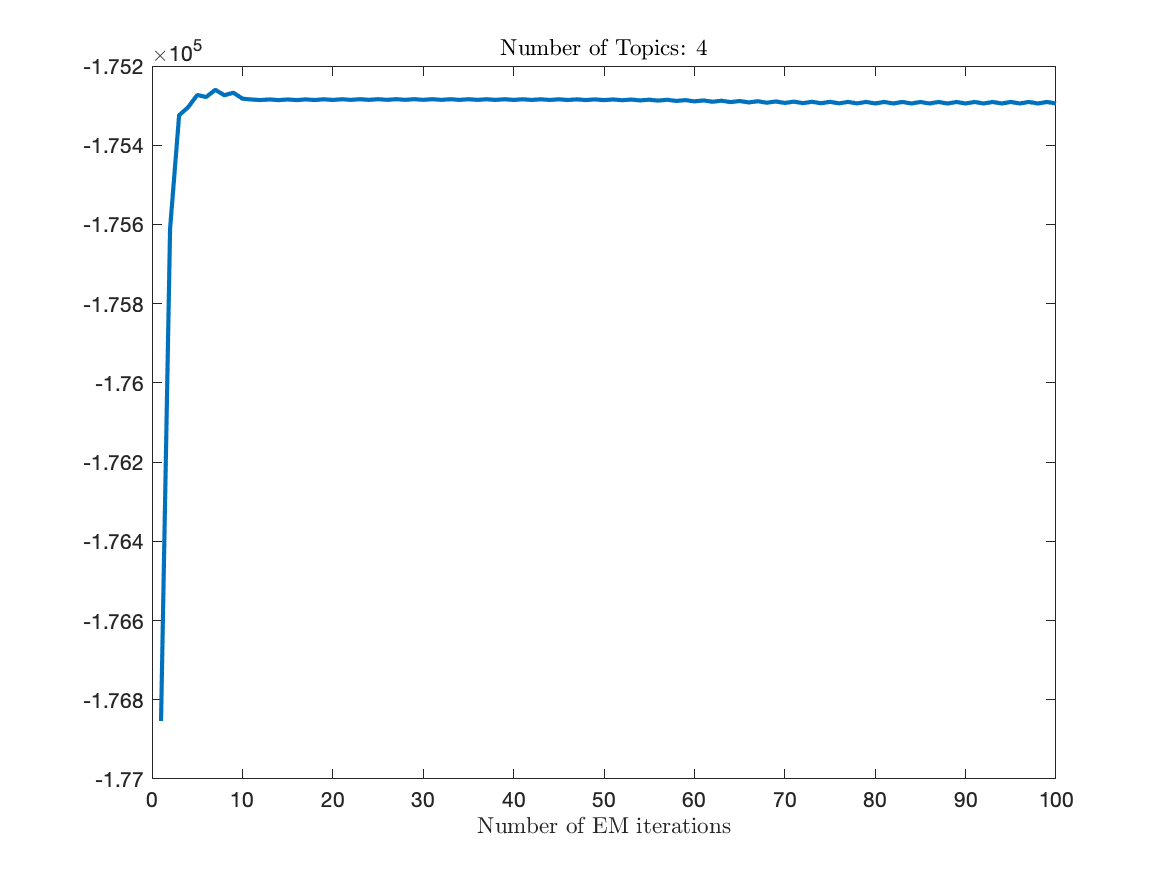
\includegraphics[width=\textwidth]{images/Q_4_topics.png}
		\caption{Log-likelihood curve for K = 4}
		\label{fig:Q4}
	\end{subfigure}
	~	
	\begin{subfigure}{0.45\textwidth}
		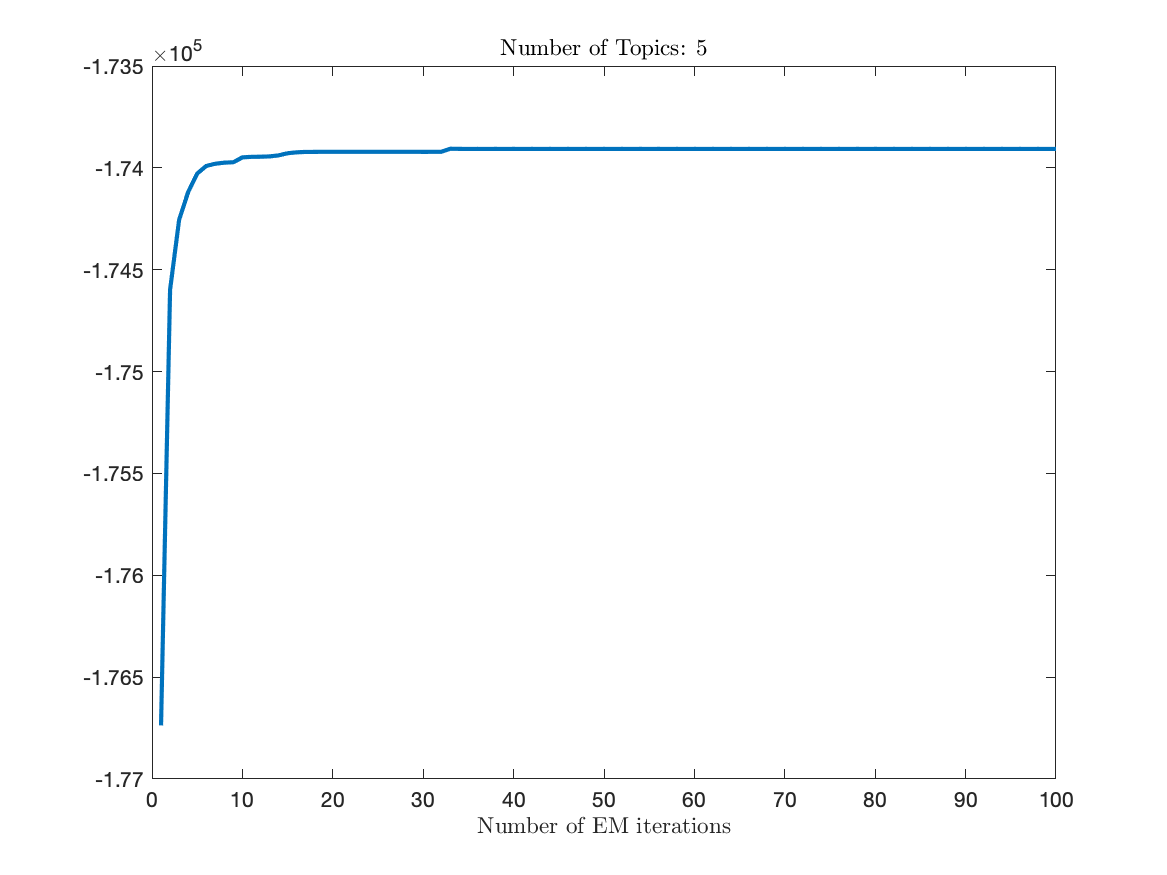
\includegraphics[width=\textwidth]{images/Q_5_topics.png}
		\caption{Log-likelihood curve for K = 5}
		\label{fig:Q5}
	\end{subfigure}
	\caption{Separated log-likelihood curves for K $\in$ [2,5]}
	\label{fig:Q_all}
\end{figure}

Finally, the states for each sequence and each document using both the MAP Forward-Backwards and the Viterbi algorithm are reported in  the Figures \ref{fig:viterbi_2}, \ref{fig:viterbi_3}, \ref{fig:viterbi_4} and \ref{fig:viterbi_5}.

\begin{figure}[h]
	\centering
	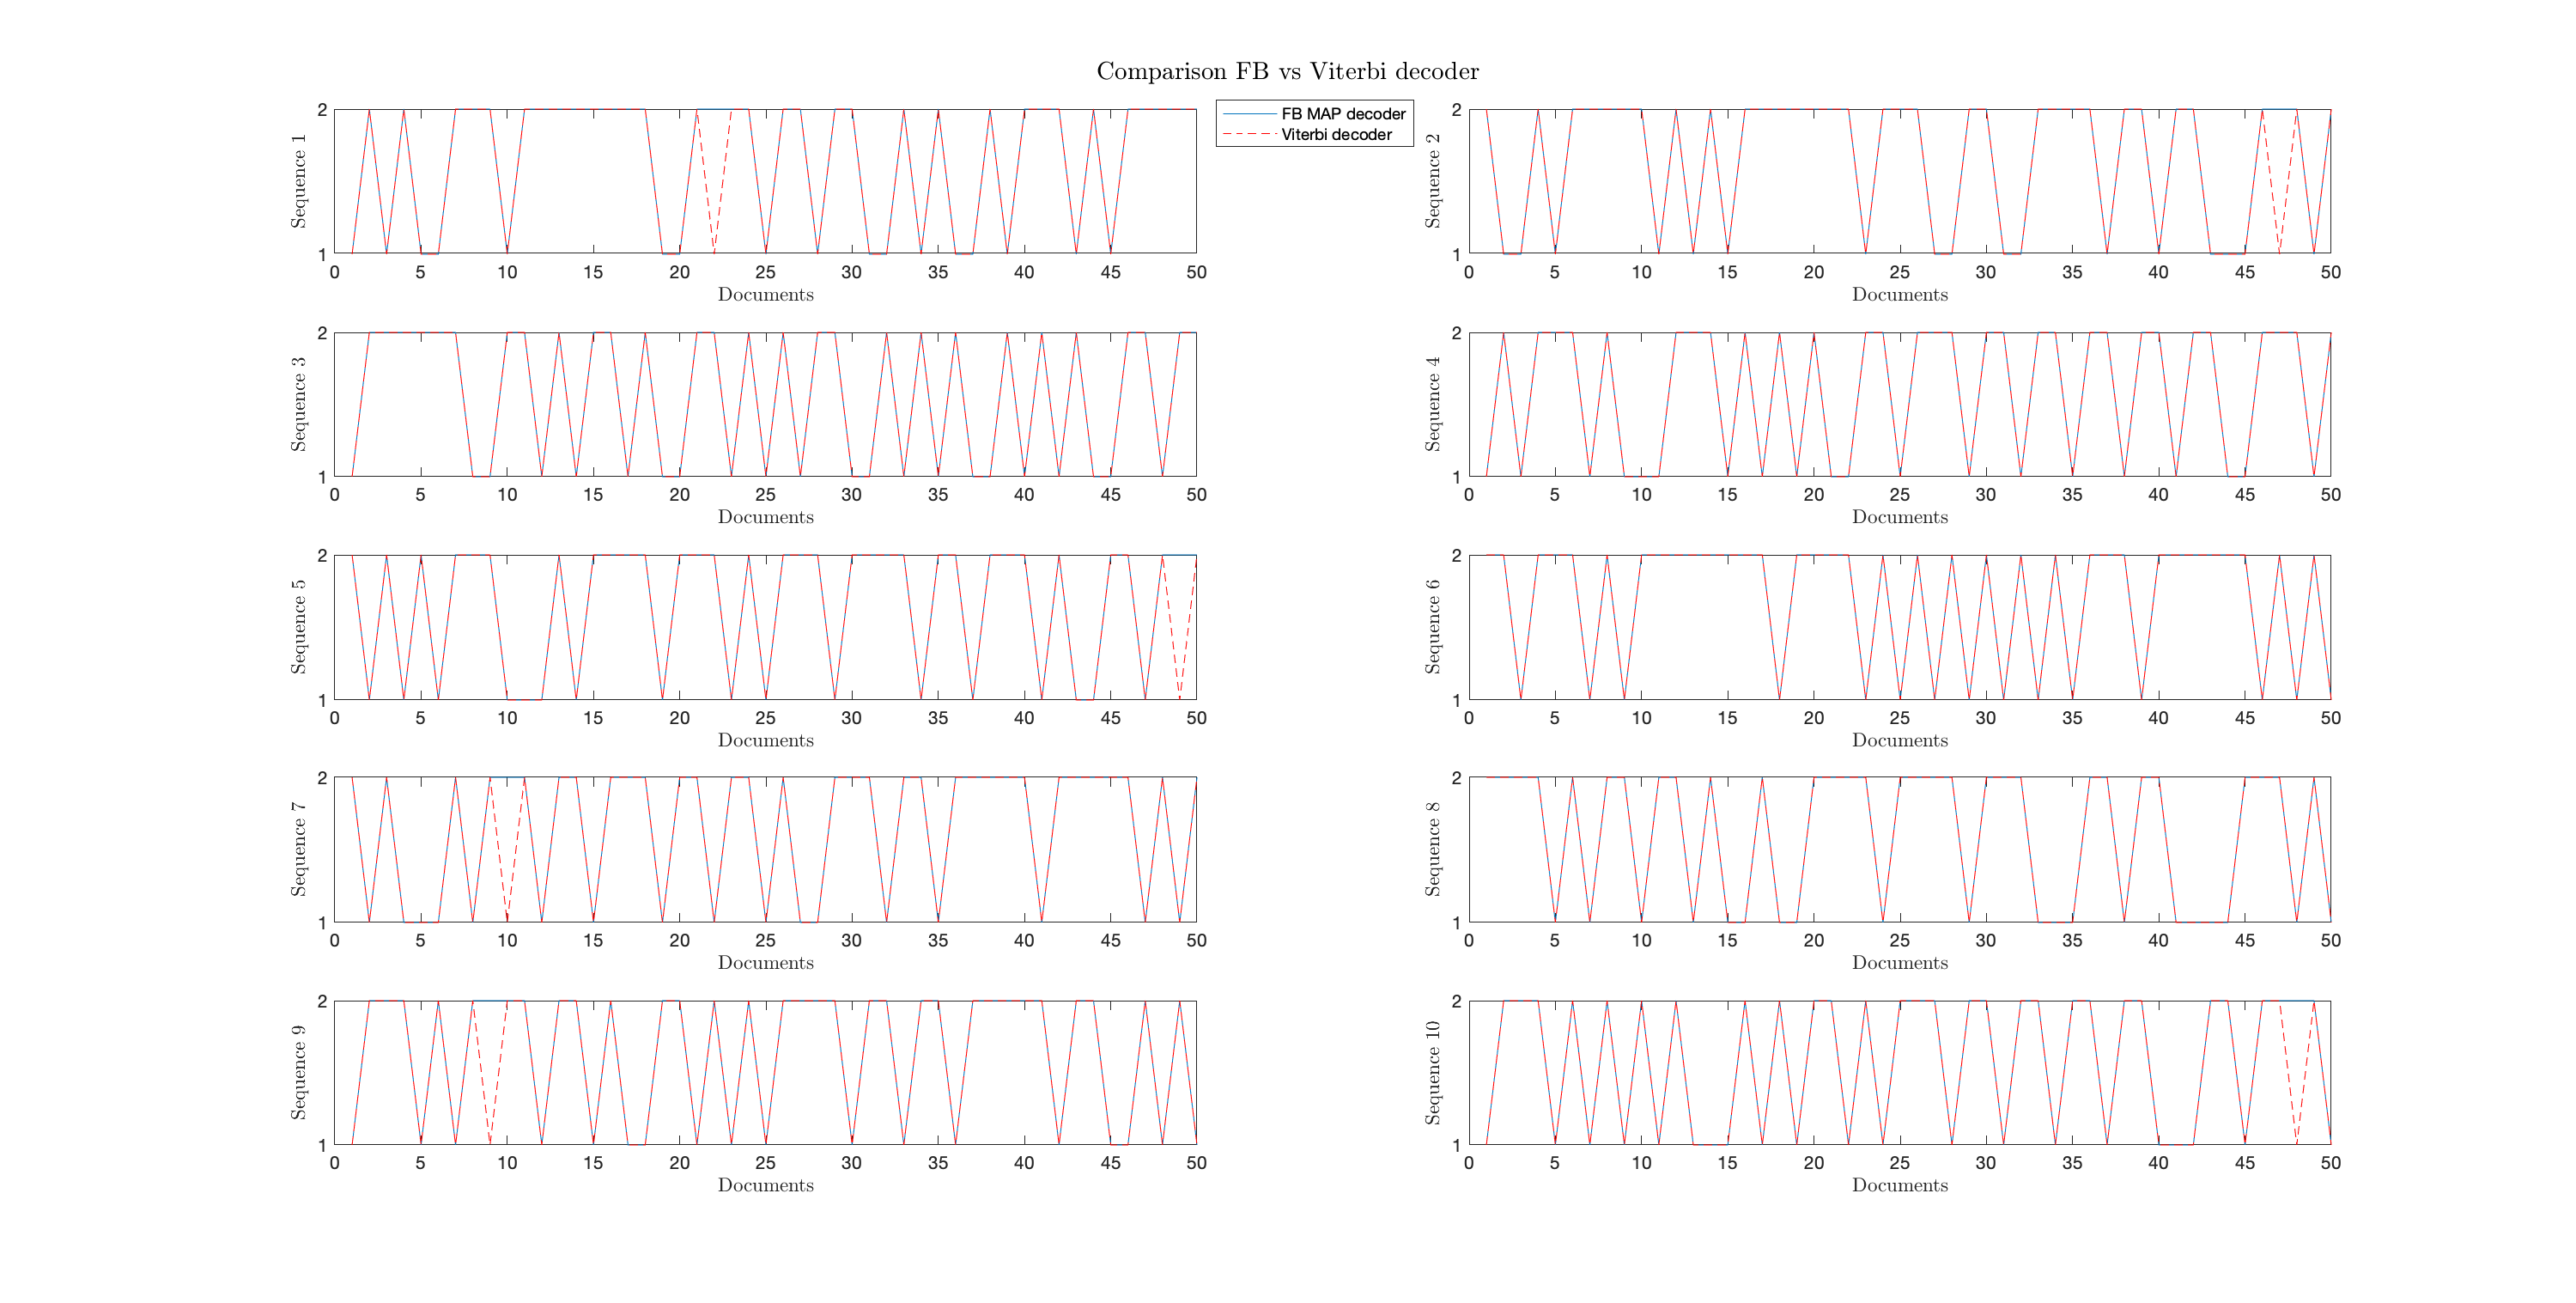
\includegraphics[width=\textwidth]{images/comparison_FB_Viterbi_K_2.png}
	\caption{Forward Backward (MAP) and Viterbi (ML) estimations for K = 2}
	\label{fig:viterbi_2}
\end{figure}

\begin{figure}[h]
	\centering
	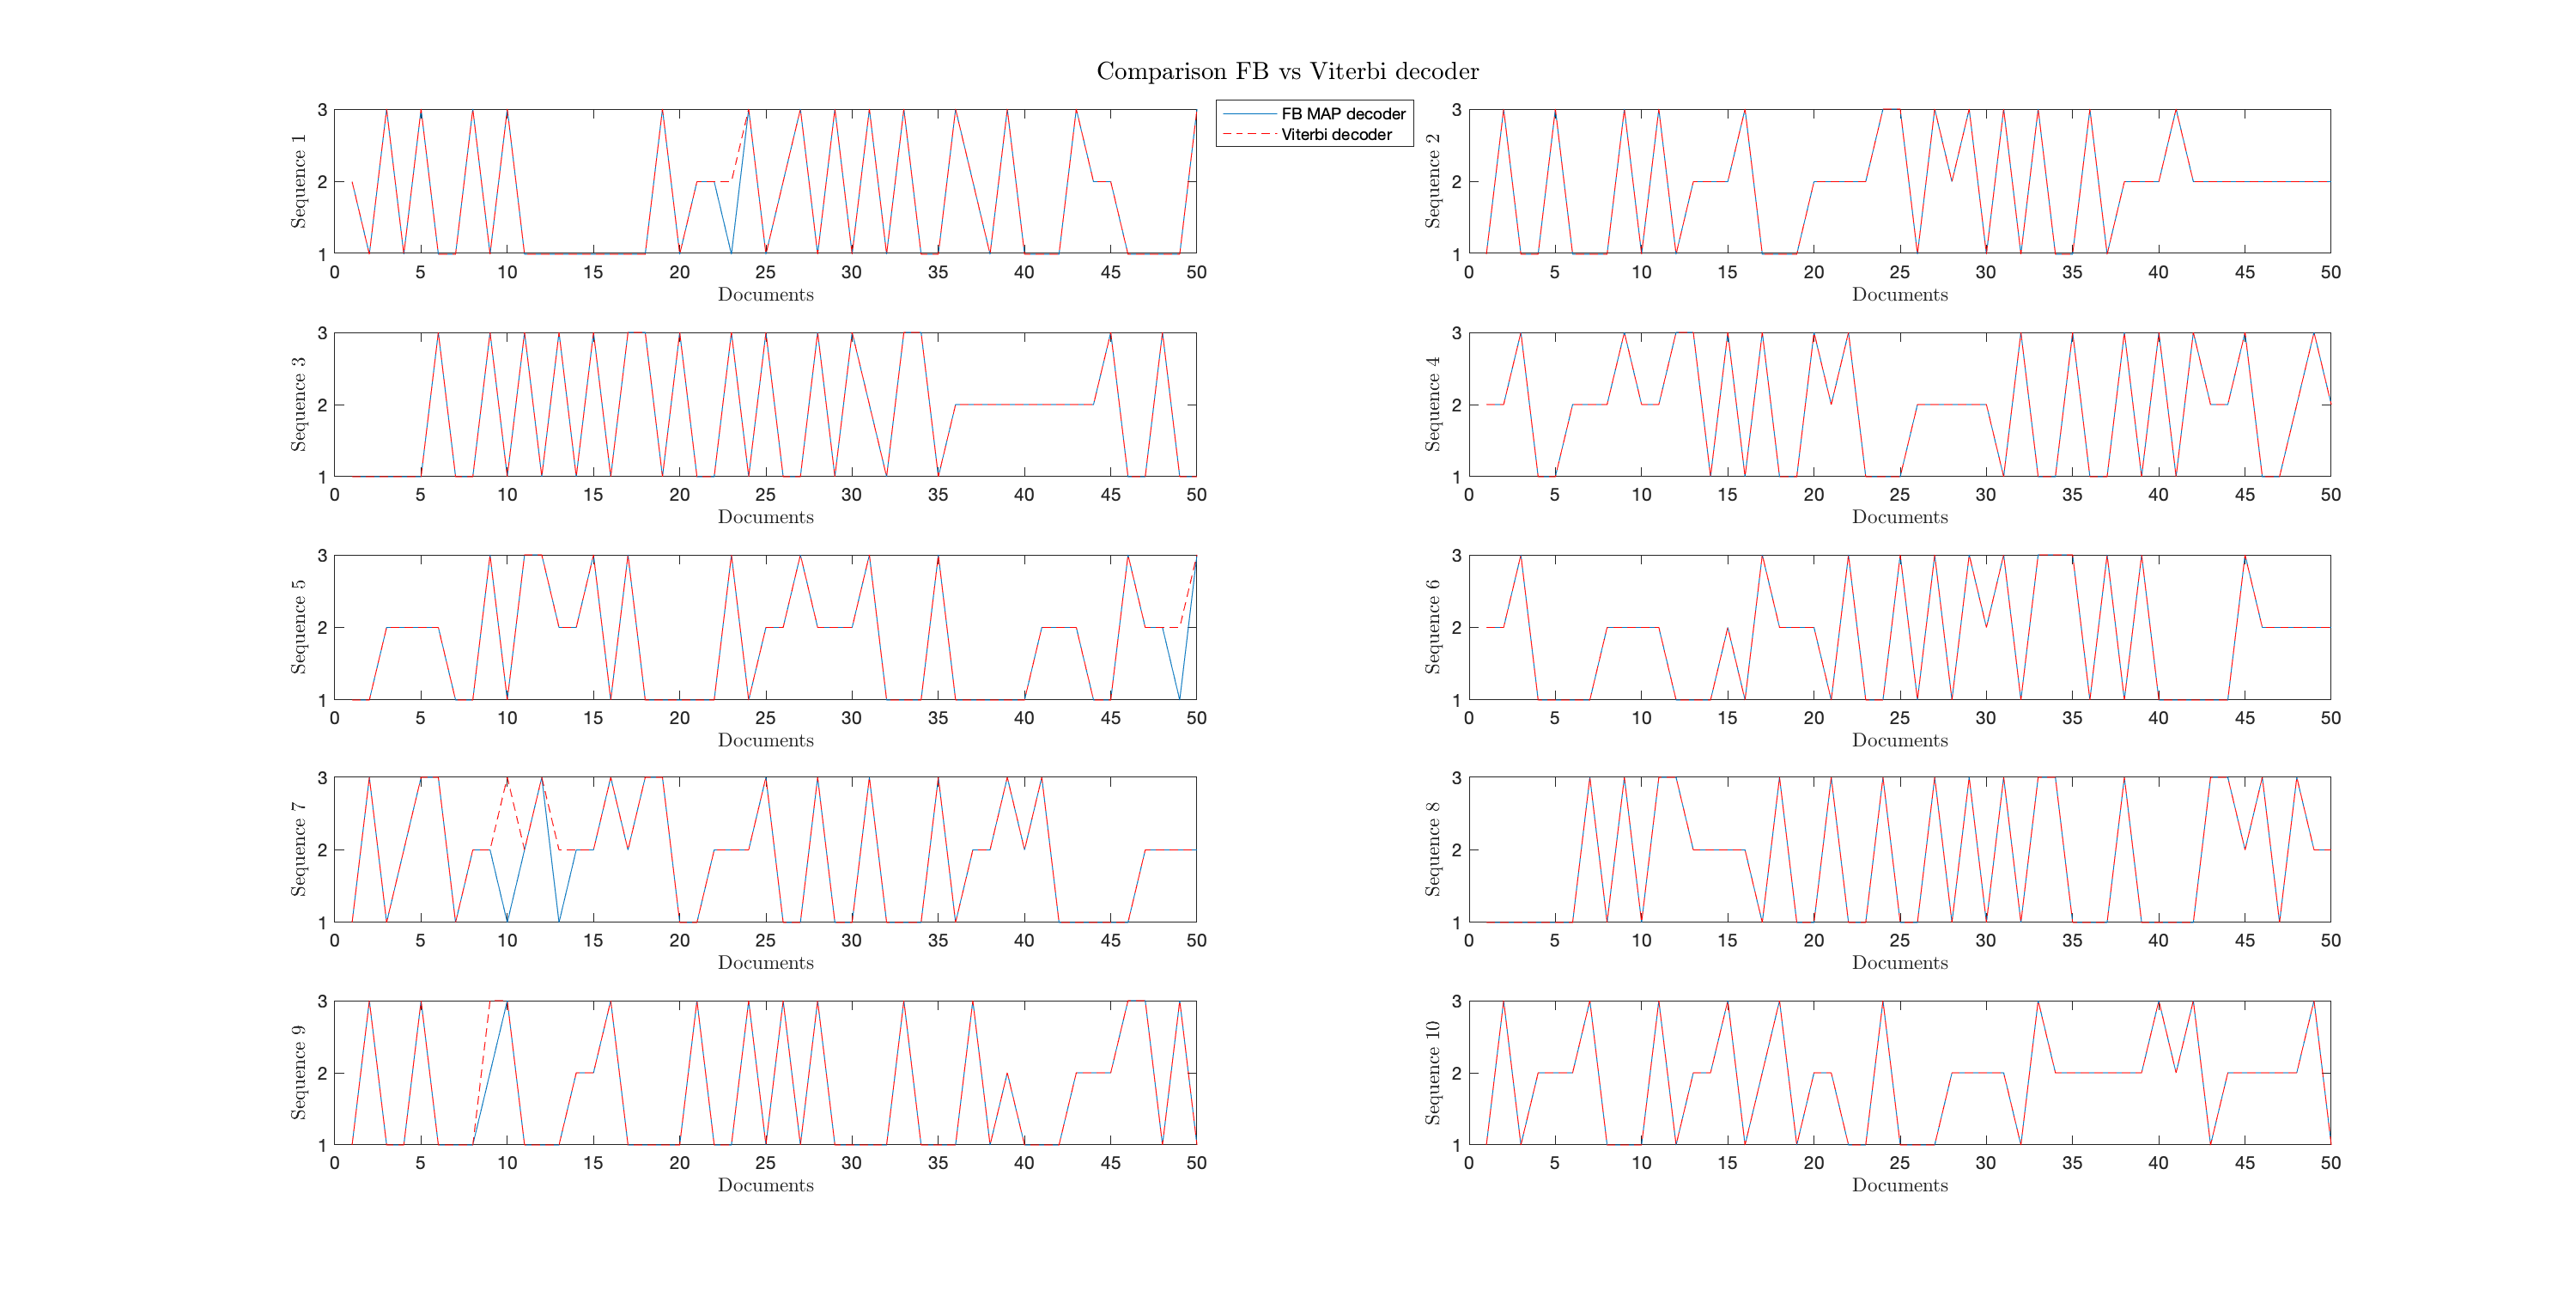
\includegraphics[width=\textwidth]{images/comparison_FB_Viterbi_K_3.png}
	\caption{Forward Backward (MAP) and Viterbi (ML) estimations for K = 3}
	\label{fig:viterbi_3}
\end{figure}

\begin{figure}[h]
	\centering
	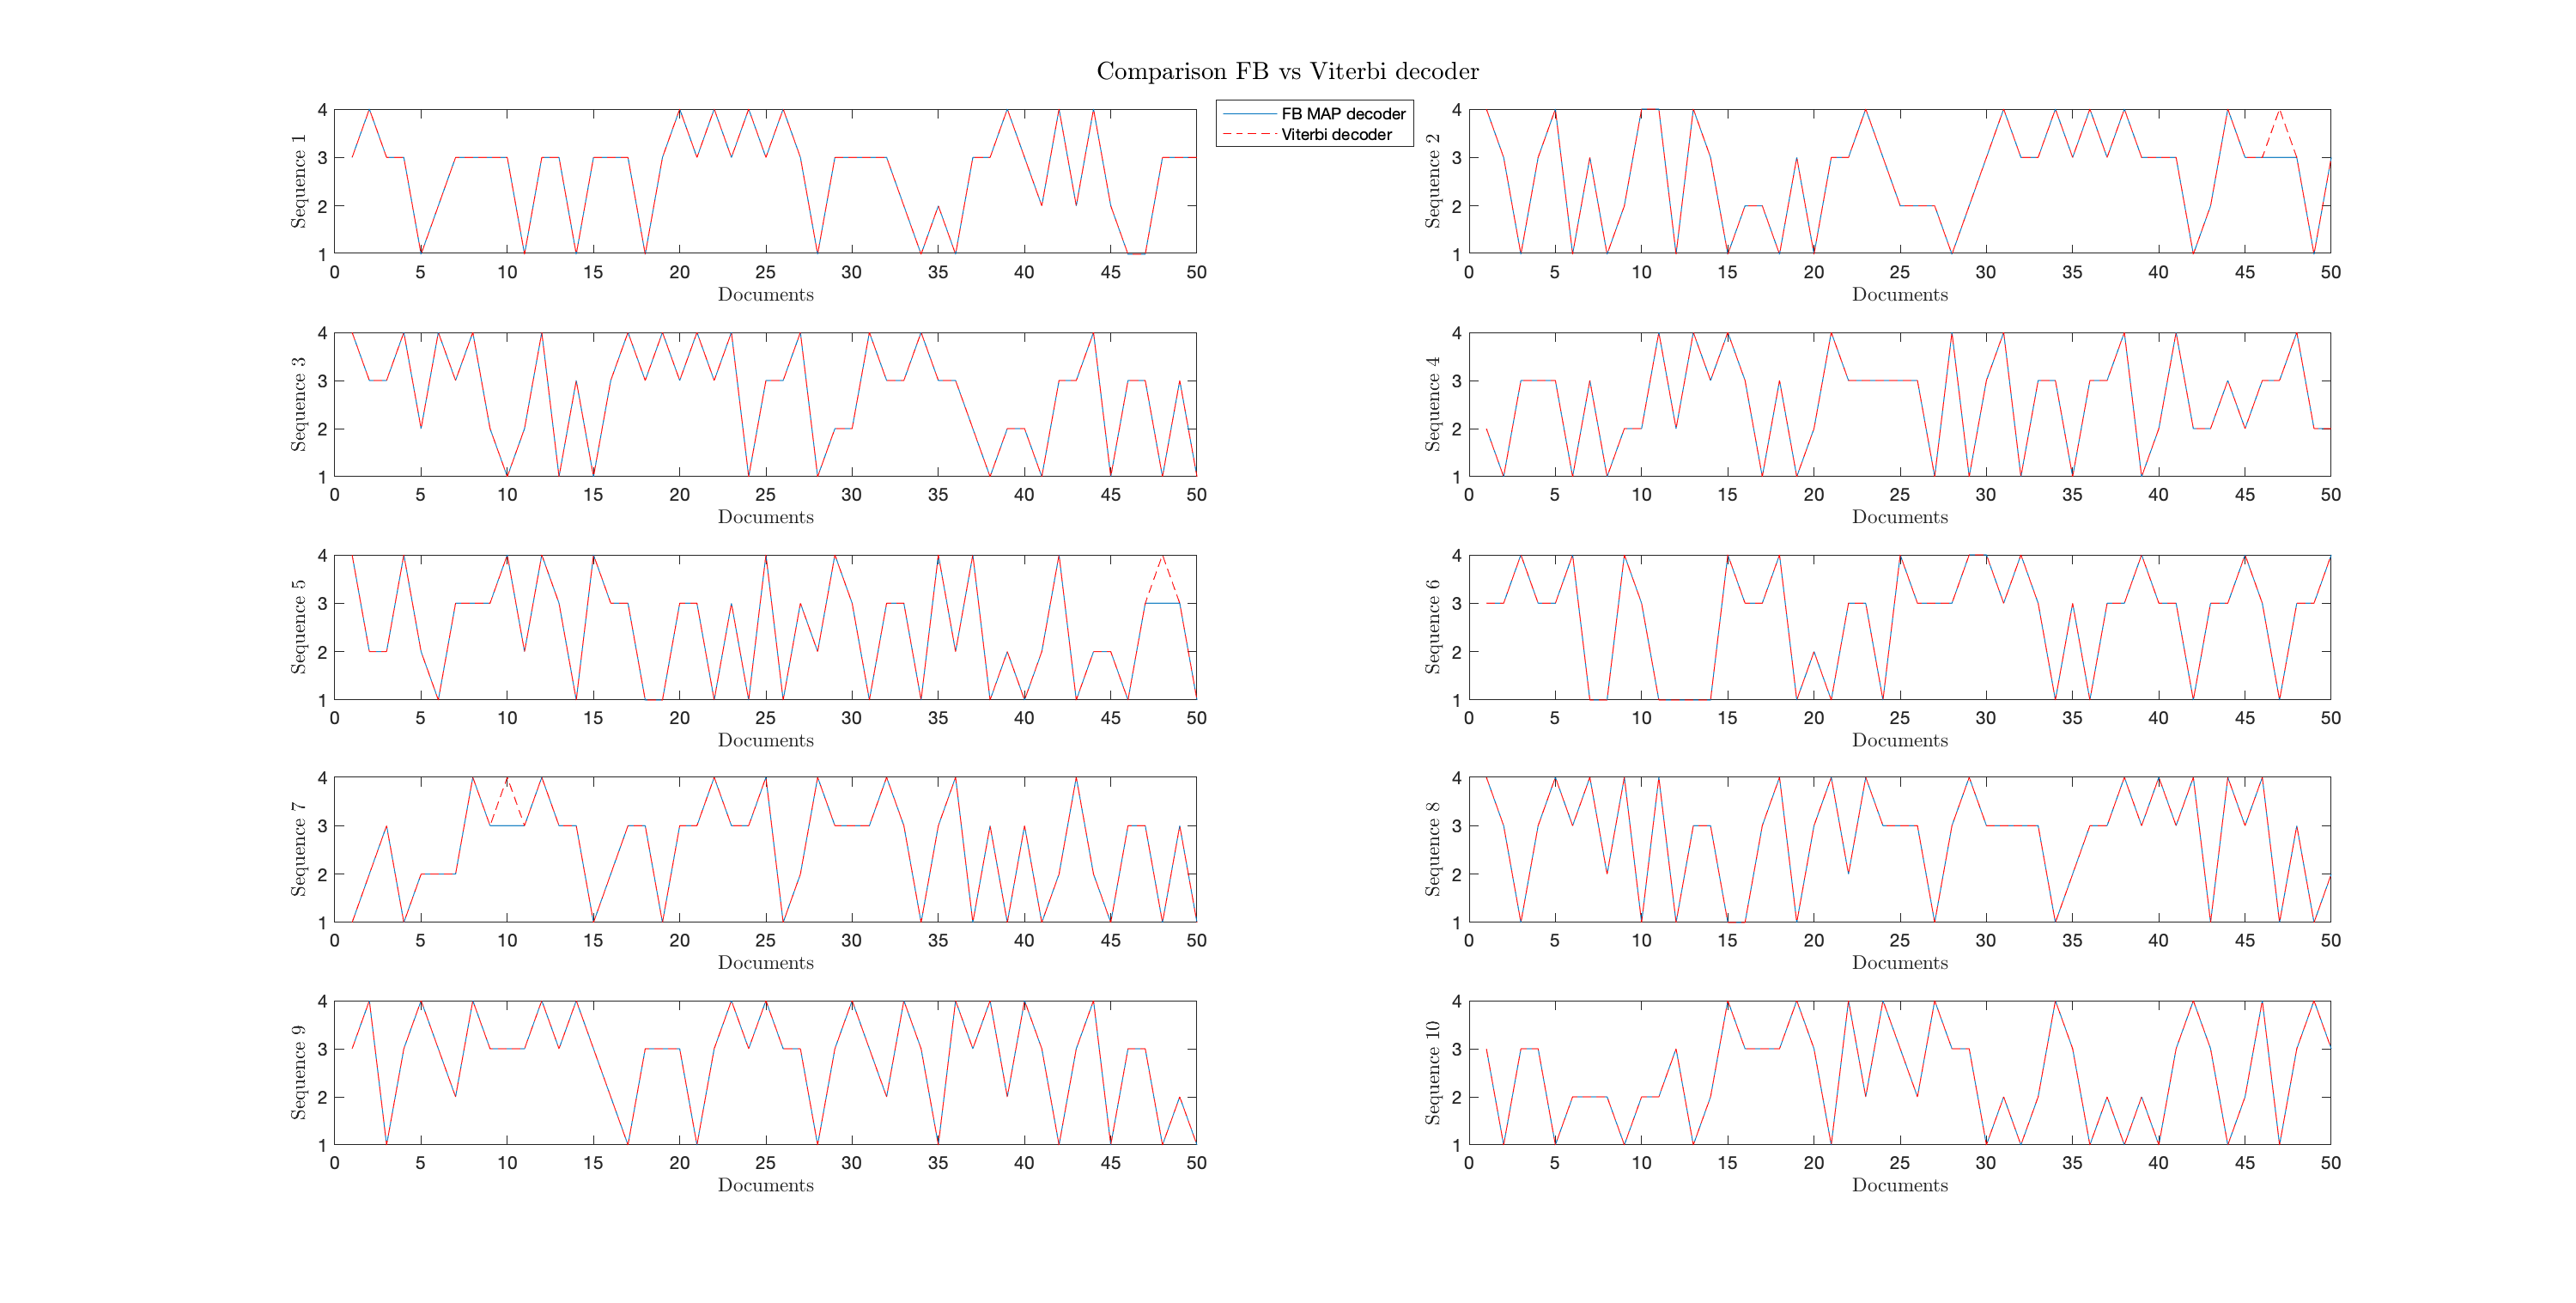
\includegraphics[width=\textwidth]{images/comparison_FB_Viterbi_K_4.png}
	\caption{Forward Backward (MAP) and Viterbi (ML) estimations for K = 4}
	\label{fig:viterbi_4}
\end{figure}

\begin{figure}[h]
	\centering
	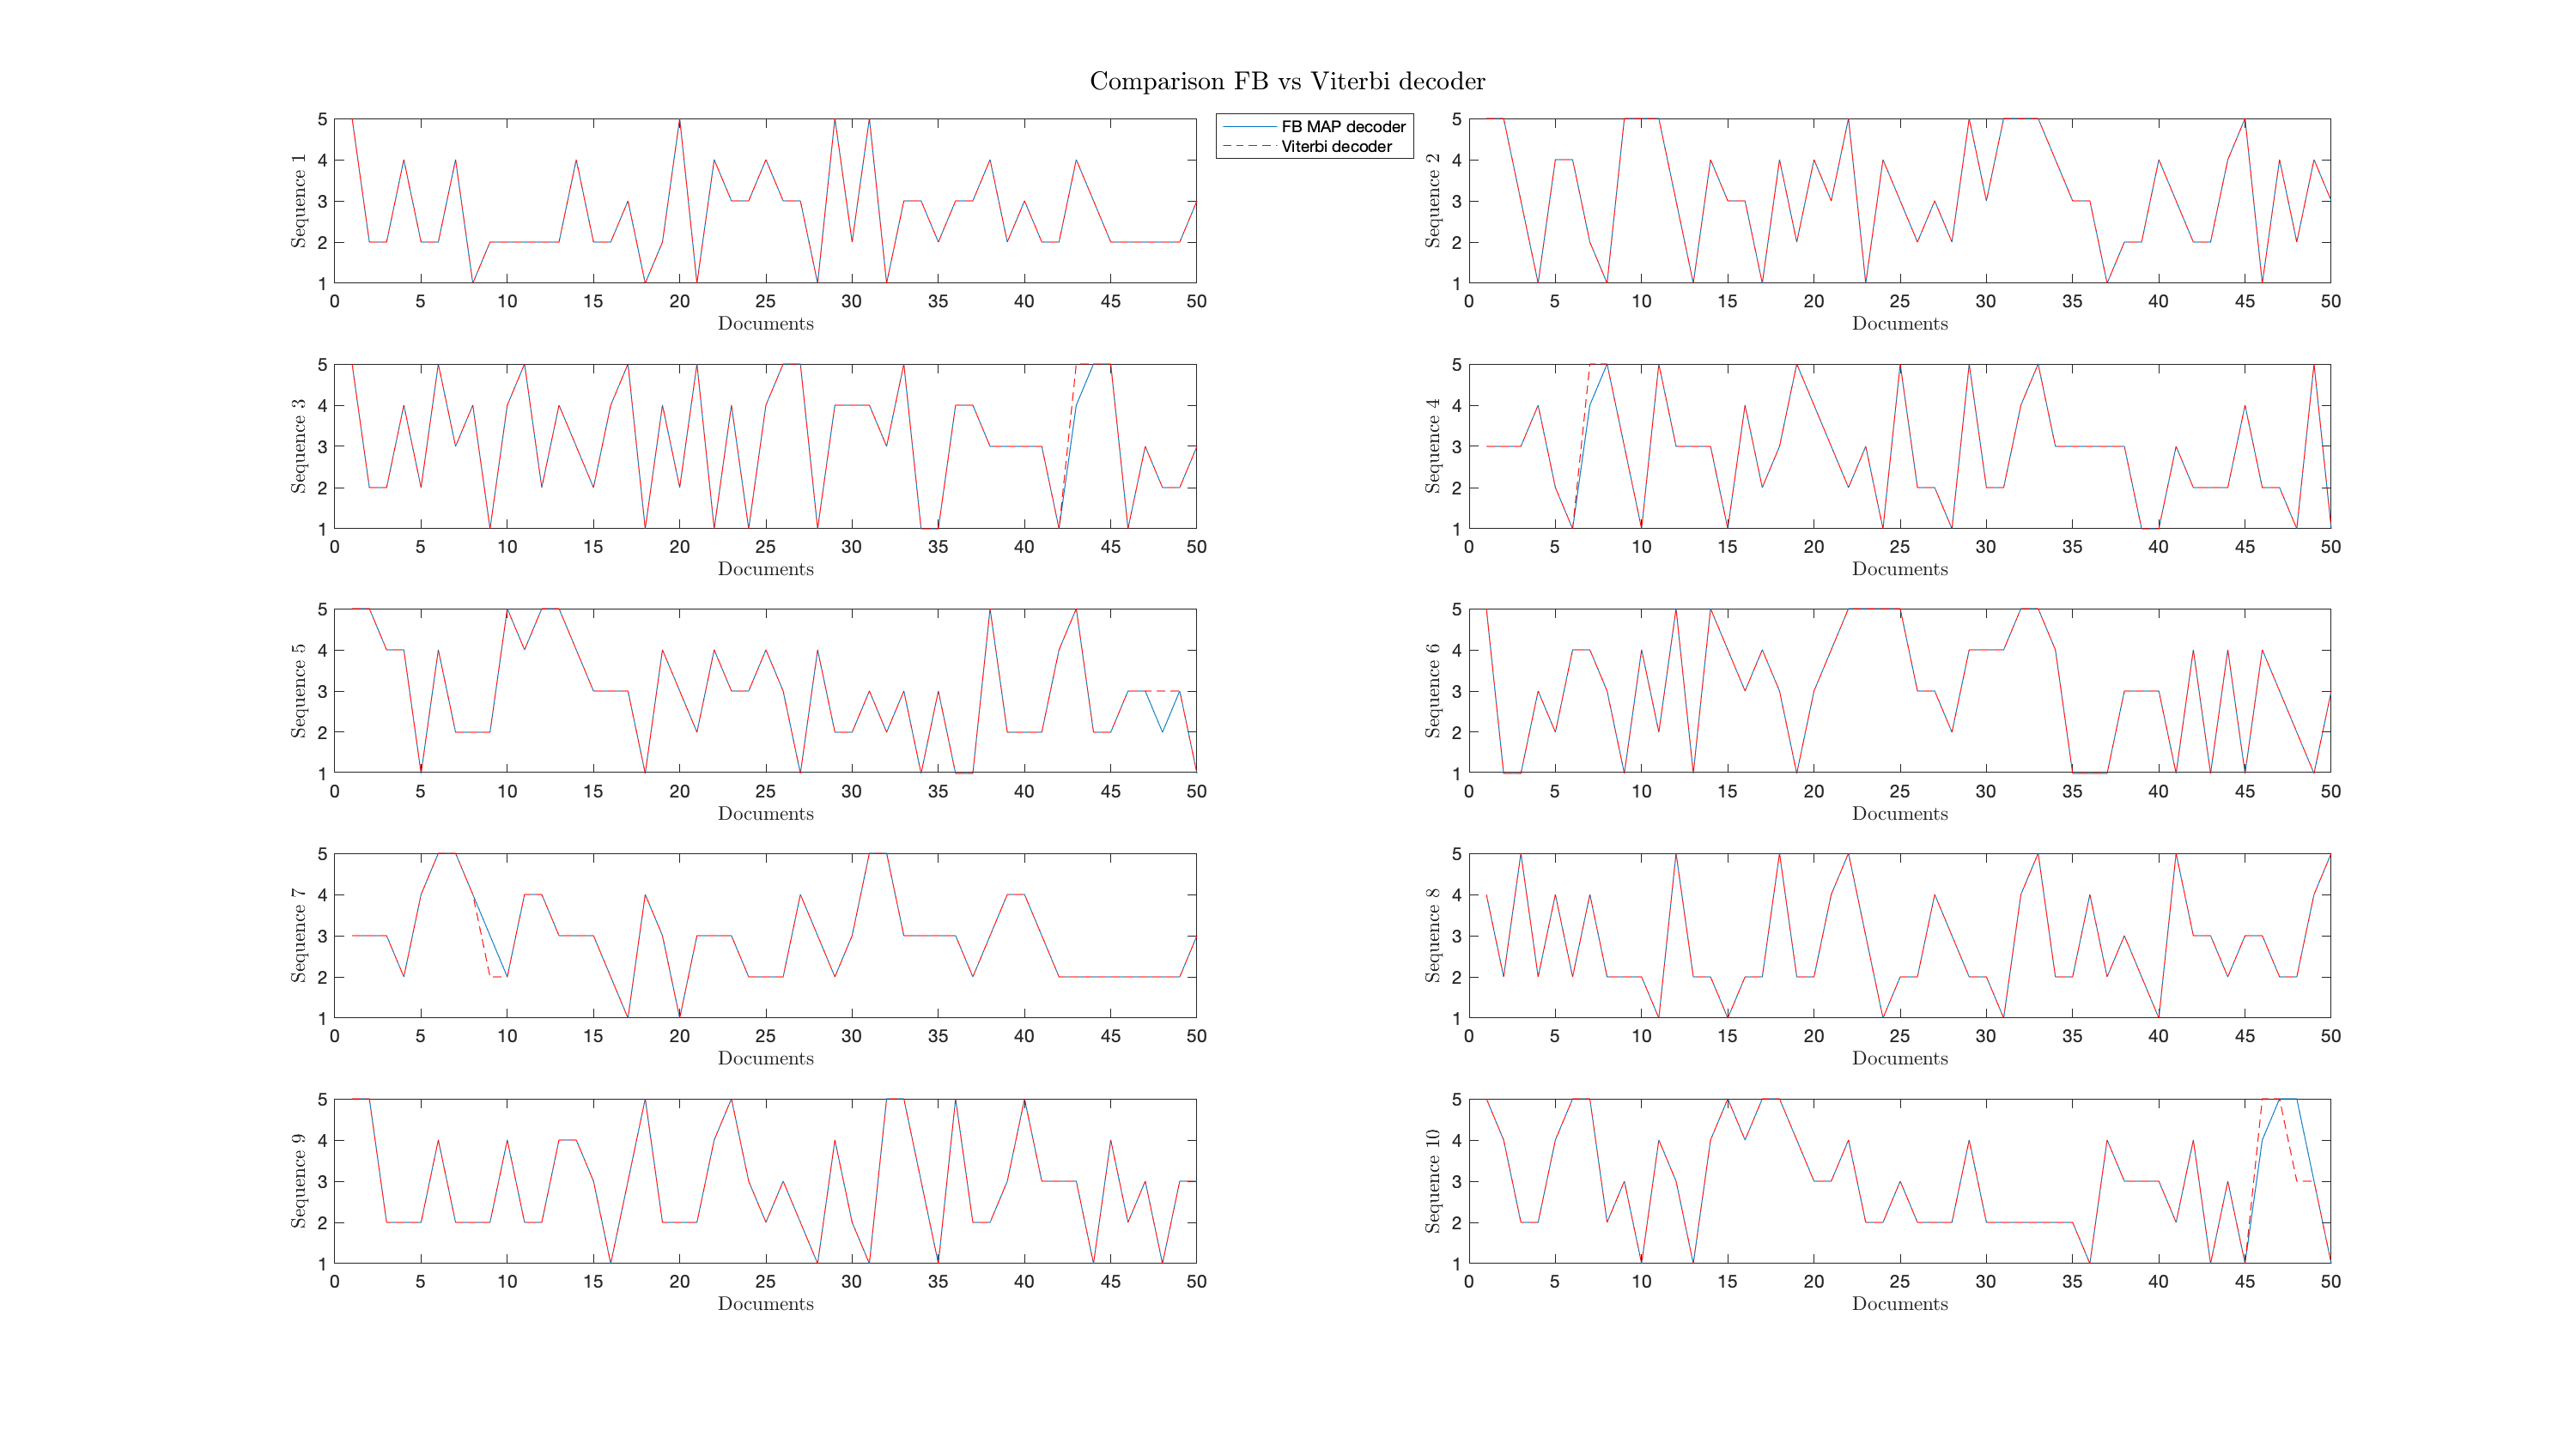
\includegraphics[width=\textwidth]{images/comparison_FB_Viterbi_K_5.png}
	\caption{Forward Backward (MAP) and Viterbi (ML) estimations for K = 5}
	\label{fig:viterbi_5}
\end{figure}

\section{Conclusions}
In this project we have implemented the EM Baum-Welch algorithm to apply it on a sequence of documents in order to find the topics they belong to. This is done using a HMM approach, for which we have been able to see the different states using the MAP state-by-state Forward-Backwards decoder and the Viterbi algorithm.
Although our final reported likelihoods had some oscillations, still we could check that the likelihood improves at every iterations, and the final output with the model parameters is consistent to the solution we were looking for. However, we have not been able to compare the results of the decoding to the ground truth solution and therefore we cannot be certain whether the optimal number of topics is $K=3$ or $K=5$. What is clear is that every document is generated by a certain state and therefore it belongs to a very specific topic.
\clearpage
\nocite{*}
\printbibliography
\end{document}
